\section{External Transactions}
\label{sec:external_transactions}

\begin{figure}[H]
\centering
\includegraphics[scale=0.48]{08_external_transactions/png/external_transactions}
\caption{External Transactions}
\label{fig:external_transactions}
\end{figure}

Figure \ref{fig:external_transactions} shows an external transaction. Without some extra form of
coordination, implemented by some additional accounts, the transaction as it stands in the figure
would be very difficult to coodinate. But it captures the important property of external
transactions, that across the market boundaries the exchange rate is the rate of payments in
currency $A$ as a ratio of the rate of payments in currency $B$.

\[
    X = \frac A  B
\]


where $X$ is the exchange rate and the unit is

\[
    \left[ \frac {\$} {yen} \right]
\]

Following our program, we'll look at how external transactions interact with other transaction
types.

\subsection{External Transactions and Exchange Transactions}

\begin{figure}[H]
\centering
\includegraphics[scale=0.48]{08_external_transactions/png/external_and_exchange_tx}
\caption{Interaction of External and Exchange Transactions}
\label{fig:external_and_exchange_tx}
\end{figure}

There is a negative feedback stabilizing process that brings the exchange rate into equilibrium with
the relative price levels of the two currencies. This process was described by Cassel
\cite{cassel1914} in 1914. If   

\[
    \frac {P_A} {P_B} > \frac A B
\]

the goods and services in currency $B$ are cheaper than goods and services in currency $A$, and so
exports of goods and services from $B$ to $A$ increase, and exports of goods and services from $A$
to $B$ decrease. This process continues until an equilibrium where

\[
    \frac {P_A} {P_B} \dot{=} \frac A B
\]

where $\dot{=}$ represents the equilibrium state.

\subsection{External Transactions and Time Transactions}

Because time transactions also involve the exchange of goods and services, time transactions also
contribute to the stabilization process described in the previous section. Repayments across the
external transaction market are determined in earlier periods from short term to long term
contracts, and therefore do not have the equilibriating ``power'' that exchange transactions do.
Interest rate differentials across the two currencies are liable to cause unpredictable disturbances
across the two currencies.

\subsection{External Transactions and Contract Transactions}

Contract transactions are only minimally connected to an initial exchange transactions, but can
involve multiple and continuing payments for changes in contract status. This proces is liable to
cause strong disturbances unrelated to the equilibriating process, and therefore are highly likely
to introduce disturbances to the exchange rate equilibriating process. Exchange rates across legacy
currencies that have floating exchange rates can and often do experience rapid fluctuations in
exchange rates.

\subsection{Control of External Exchange}

If only exchange transactions are allowed as external transactions the exchange rate should
equilibriate to the relative prices levels of the two currencies, otherwise know as purchasing power
parity. The introduction of contract transactions are highly likely to cause disturbances to both
currencies, making it difficult to maintain macro-equilibriation goals. Time transactions, represent
a middle-ground between contract and exchange transactions. 
